\documentclass[UTF8]{ctexart}
\usepackage{shumo}%可以点开查看宏包和定义内容，同时可以自行另外加宏包和定义
\usepackage{booktabs}
\geometry{left=2.50cm,right=2.5cm,top=2.50cm,bottom=2.5cm}%页面布局集训标准，可自行适当修改
%====================================================
%设置附录代码的格式，可以自行修改
\lstset{
	breaklines=true,% 允许自动断行
	% breakatwhitespace=true,% 使用此命令仅允许在空格处自动断行
	showstringspaces=false,% 不显示字符串中的空格
	basicstyle=\small\ttfamily,% 设置代码基本样式
	flexiblecolumns=true,% 改善字母间距
	keywordstyle=\color{blue},% 设置关键词样式
	stringstyle=\color[rgb]{0.75,0,0.75},% 设置字符串样式
	commentstyle=\songti\color[rgb]{0,0.5,0},% 设置注释样式
	tabsize=4,% 设置制表符缩进
}
%====================================================
\title{\textbf{杭电数学建模竞赛}}% 请勿修改
\date{}%请勿添加自己的信息
\author{}%请勿添加自己的信息
%下面时正文
\begin{document}
\setcounter{page}{1}%从正文开始计算页码	
\maketitle
\vspace{-0.95cm}
\thispagestyle{fancy}   
\fancyhf{} %清除原本页眉页脚形式
\renewcommand{\headrulewidth}{0pt} %页眉线宽，设为0可以去页眉线
%=================================================
%=================================================
%=================================================
%=================================================
%=================================================
%=================================================
%下面开始出现各位需要修改的部分。
\renewcommand{\abstractname}{\sihao 摘\quad 要} %更改摘要二字的样式
\begin{abstract}\xiaosihao
	\vspace{0.1cm}
	以下只是一个样例说明，通过下面说明各位同学可以进行学习如何换行，加粗字体。预祝各位同学取得好成绩！\par
	针对问题一，分析商品买卖机理，\textbf{建立基于双十一规则商家利益最大化判别模型}。本文以经济学价格理论为基础，分析得商家参与活动通过降低单次商品利润提高总销量而获得更高利润。\textbf{选取利润为指标}，基于商家参与活动规则，综合活动前后利润判别式，以营业额最大化为目标建立判别模型。通过具体数据如WIS水润面膜相对非双十一销售额翻了近110倍说明商家是理性的。\par
	针对问题三，分析选取消费者与商家群体双赢指标，\textbf{建立消费者是否购买与商家是否提供高质量服务的演化博弈模型}。本文考虑商家与消费者对“赢”的定义不同，查阅文献\textbf{以商家能吸引消费者购买和消费者能得到高质量服务为双赢指标}。基于不同行为下商家与消费者收益变化，建立演化博弈模型。\textbf{模型求解结果为消费者趋向于购买和商家趋向于提供高质量服务的双赢局面}，并通过2009-2019年成交总额的指数型上涨说明结果准确性。\par
		针对问题三，分析选取消费者与商家群体双赢指标，\textbf{建立消费者是否购买与商家是否提供高质量服务的演化博弈模型}。本文考虑商家与消费者对“赢”的定义不同，查阅文献\textbf{以商家能吸引消费者购买和消费者能得到高质量服务为双赢指标}。基于不同行为下商家与消费者收益变化，建立演化博弈模型。\textbf{模型求解结果为消费者趋向于购买和商家趋向于提供高质量服务的双赢局面}，并通过2009-2019年成交总额的指数型上涨说明结果准确性。\par
	针对问题四，基于商家竞争规律，\textbf{建立商家是否提供高质量商品的演化博弈模型}。考虑到电子商务普遍有商品质量不高现象，\textbf{本文以双十一作用下商家间竞争能否提高商品质量为指标}。基于不同行为下同类商家收益变化建立模型。\textbf{模型求解结果为同类商家之间趋向用高质量商品进行竞争}，通过2013-2015年双十一过后的投诉率（$6.9$、$6.1$、$4.6\times10^{-7}$）不断下降说明结果准确性。\par
	针对问题五：本文从商家和买家的角度考虑，在前面四问的基础上，以国家质检局抽检网络产品不合格率以及双十一个人网购数据为例对双十一购物期间某些不理性的行为进行说明，并提出\textbf{“理性消费”}的合理建议，即：\textbf{商家销售保持诚信}、\textbf{买家购物理性消费}、\textbf{买家积极反馈维权}。
	\\
	
	%这里填写你自己的关键词
	
	\textbf{关键词}:\quad 双十一购物节，基于目标规划的判别模型，演化博弈模型
\end{abstract}

\pagestyle{plain}
%标准 LaTeX 提供下列四种页版式，可用 \pagestyle{页版式} 命令来设置页面版式：
%empty(没有页眉和页脚)，plain(本次用的，无页眉，页脚为居中页码)，headings(页眉为章节标题，无页脚)，myheadings(页眉内容可自定义，无页脚)
\newpage

\section{问题重述}
\subsection{问题背景}
异形圆管工件广泛应用于装备制造、汽车零部件及工业管路等领域。实际生产中，企业通常采用激光切割方式从标准圆管母材中加工所需工件。由于不同工件的几何形状和轴向占用长度不同，若母材选取和下料顺序安排不合理，将导致母材浪费增加、利用率降低，从而影响企业生产成本和加工效率。

与普通一维下料问题相比，异形圆管工件下料还存在端部共切和加工切换等实际因素。相邻工件若能选择合适的端部拼接方式，可减少中间多余切割区域，提高材料利用率；同时，同类工件连续加工有利于降低排产和现场操作复杂度。因此，如何在满足生产需求的前提下，综合考虑母材选取、工件排序、端部拼接和余料利用，制定高效的下料方案，具有重要的实际意义。
\begin{figure}[H]
	\centering
	
\includegraphics[width=0.62\textwidth]{1.png}
	\caption{工件切割示意图}
	\label{fig:单图}
\end{figure}
\subsection{问题提出}
针对上述生产背景，本文需要围绕异形圆管工件的下料与拼接优化建立数学模型，并逐步解决以下问题。

\textbf{问题一}：在不考虑共切效应的情况下，根据 10 类工件的三维离散坐标数据计算各类工件的轴向占用长度，并在每类工件需求量均为 50 件、母材长度可选的条件下，确定母材选取和基础下料方案，使所选母材总长度尽可能小。

\textbf{问题二}：在问题一所得下料方案基础上，考虑相邻工件端部之间的共切效应，计算不同工件对在四种端部组合下的共切收益。在保持各工件分配到各母材不变的条件下，重新优化每根母材内部的加工顺序和拼接方式，使总共切收益尽可能大，并尽量减少工件切换次数。

\textbf{问题三}：在考虑共切收益的基础上，不再固定问题一中的母材分配方案，而是对母材选取、工件分配、加工顺序和端部拼接方式进行联合优化，建立综合下料模型，使母材总长度尽可能小、总共切收益尽可能大、总切换次数尽可能少。

\textbf{问题四}：将模型推广到 3 个连续加工批次，结合余料入库及优先使用原则，确定各批次的余料调用、新母材选取、工件拼接方式和加工顺序，实现多批次整体下料方案的优化。
\section{问题分析}
\subsection{问题1的分析}
针对问题一，首先需要计算各工件的轴向占用长度，并据此建立模型。因为题目暂不考虑共切收益，可以将工件简化为其空间最小外接包围盒（OBB）。为计算工件轴向长度，需要先确认轴的位置，而后计算其轴向投影长度。在得到 10 类工件的单件长度后，可将每类 50 件工件视为待放入母材的物品，将 9m、10m、11m、12m 四种标准母材视为可选箱体，建立一维下料优化模型。该问题的主要目标是使所选母材总长度最小，在此基础上统计各根母材的工件顺序、母材利用率和不同工件之间的切换次数。
\subsection{问题2的分析}
针对问题二，在问题一的基础上，需要对每根母材内部工件的加工进行重新排序，并进行工件拼接。由于相邻工件端部之间可能存在共切效应，任意两件工件在 LL、LR、RL、RR 四种端部组合下的共切收益可能不同，因此需要根据工件端部几何形状建立省料计算模型，得到工件对之间的共切收益矩阵。在此基础上，每根母材内部的排序问题可转化为带边权的路径优化问题：节点表示已分配到该母材上的工件，边权表示相邻工件采用某种端部组合时的共切收益。求解时应优先最大化总共切收益，并在收益相同或接近时尽量减少不同类型工件之间的切换次数。
\subsection{问题3的分析}
针对问题三，不再固定问题一中的母材分配方案，而是将母材选取、工件分配、加工顺序和端部拼接方式统一纳入优化过程。与问题二相比，问题三的决策空间明显增大，因为工件不仅可以在同一母材内部重新排序，还可以重新分配到不同母材中。此时模型既要保证每根母材上的实际占用长度不超过其标准长度，又要考虑相邻工件拼接产生的共切收益。由于题目要求母材总长度最小为主要目标，共切收益最大为次要目标，切换次数最少为再次目标，因此可采用分层优化思想：首先确定母材总长度最小的可行方案，再在该方案集合中寻求共切收益较大的排序与拼接方式，最后进一步优化工件切换次数。
\subsection{问题4的分析}
针对问题四，模型需要从单批次下料扩展到连续 3 个批次的动态优化。该问题的难点在于余料具有跨批次传递特征：当某批次加工结束后剩余母材长度不小于 0.2m 时，可作为余料入库并在后续批次中优先使用；若不足 0.2m，则视为废料。因此，问题四不仅要分别优化每个批次内部的母材选取、工件排序和拼接方式，还要考虑前一批次余料对后一批次可用材料集合的影响。可将每个批次看作一个阶段，将可用余料状态作为阶段间传递信息，建立多批次动态下料优化模型。在求解目标上，仍应保持母材总长度最小的优先级，同时兼顾总共切收益和总切换次数，从而得到符合企业实际生产逻辑的连续加工方案。
\section{假设与符号说明}
\section{数据预处理}
本节对原始三维测绘点云数据进行必要的降重与异常值检测，保证后续轴向长度计算与下料模型建立的输入质量。

\subsection{重复值检测与去重}

首先对每个工件的原始点集进行了重复点检测与去重（降重），去重后点数及异常值检测结果汇总见表\ref{tab:dedup}。
\begin{table}[htbp]
\centering
\caption{点云去重统计表}
\label{tab:dedup}
\begin{tabular}{l r r r r}
\toprule
文件名 & 原始点数 & 去重后点数 & 重复点数 & 去重容差(m) \\
\midrule
圆管1.csv  & 808  & 800  & 8    & 0.0000001 \\
圆管2.csv  & 808  & 800  & 8    & 0.0000001 \\
圆管3.csv  & 2020 & 2000 & 20   & 0.0000001 \\
圆管4.csv  & 1818 & 1800 & 18   & 0.0000001 \\
圆管5.csv  & 1224 & 204  & 1020 & 0.0000001 \\
圆管6.csv  & 876  & 146  & 730  & 0.0000001 \\
圆管7.csv  & 684  & 114  & 570  & 0.0000001 \\
圆管8.csv  & 1176 & 196  & 980  & 0.0000001 \\
圆管9.csv  & 1536 & 256  & 1280 & 0.0000001 \\
圆管10.csv & 936  & 156  & 780  & 0.0000001 \\
\bottomrule
\end{tabular}
\end{table}

\subsection{异常值检测及处理}

为直观判断数据质量，我们绘制了各工件的离散点散点图与提供的stp文件对比图，如下图\ref{fig:pipe1_comparison}，发现测得点云主要来自工件两端切面的截面扫描（即只对器件最外端截面进行了密集采样），数据量较少，且对比观察异常值不明显。基于这一观察，本文放弃盲目采用诸如双边滤波或统计离群点剔除（SOR）等可能导致过平滑（over‑smoothing）的复杂去噪方法，以免破坏截面几何特征。

\begin{figure}[H]
	\centering
	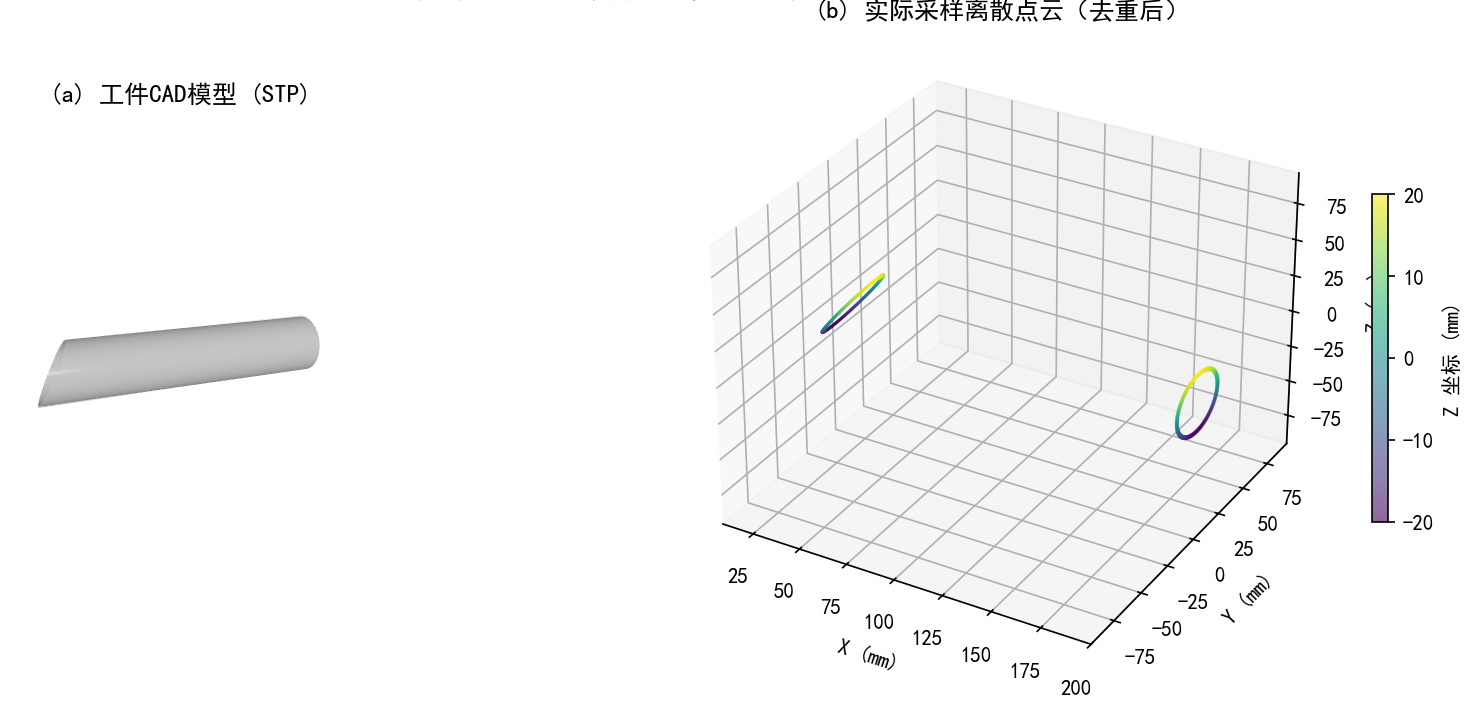
\includegraphics[width=0.62\textwidth]{圆管1_comparison.png}
	\caption{圆管1点云与STP文件对比图}
	\label{fig:pipe1_comparison}
\end{figure}
为检验是否存在异常值，将去重后数据与标准 CAD 曲面对比，采用三维空间偏差分析（3D deviation analysis）。设去重后点云为 $\{P_i(x_i,y_i,z_i)\}_{i=1}^n$，标准 CAD 数学曲面为 $\mathcal{S}$，对每个采样点 $P_i$，记其在曲面 $\mathcal{S}$ 上的最近投影点为 $Q_i^*$，曲面在 $Q_i^*$ 处的单位外法向量为 $\mathbf{n}(Q_i^*)$，
则第 $i$ 个点的有符号偏差定义为：
\begin{equation}
d_i = \mathbf{n}(Q_i^*) \cdot (P_i - Q_i^*), \qquad i=1,2,\dots,n,
\end{equation}
其中 $\cdot$ 表示向量点积。偏差的绝对值 $|d_i|$ 反映了点到曲面的距离大小，而符号 $d_i$ 的正负表示点位于曲面外部（正）或内部（负）。

对各点集计算最大绝对偏差与平均绝对偏差作为数据质量判据。表\ref{tab:summary} 列出了各文件的去重后点数、最大绝对偏差、平均绝对偏差以及是否判定为合格（清洁）。从结果可见，唯一的显著异常来自 cleaned\_圆管1（最大绝对偏差约 $437\,$mm、平均绝对偏差约 $417\,$mm），进一步核查发现该问题由单位不一致导致；其余样本的最大/平均绝对偏差均在可接受范围内。所以我们认为不存在异常值。

\begin{table}[H]
\centering
\caption{去重与异常值检测汇总（summary\_table）}
\label{tab:summary}
\begin{tabular}{lrrrc}
\toprule
文件名 & 点数 & 最大偏差(mm) & 平均偏差(mm) & 是否合格 \\
\midrule
cleaned\_圆管1  & 800  & 437.183427 & 417.400927 & 否 \\
cleaned\_圆管10 & 156  & 0.006531   & 0.001543   & 是 \\
cleaned\_圆管2  & 800  & 0.007095   & 0.001729   & 是 \\
cleaned\_圆管3  & 2000 & 0.007095   & 0.001617   & 是 \\
cleaned\_圆管4  & 1800 & 0.007095   & 0.001543   & 是 \\
cleaned\_圆管5  & 204  & 0.006216   & 0.002108   & 是 \\
cleaned\_圆管6  & 146  & 0.006238   & 0.002099   & 是 \\
cleaned\_圆管7  & 114  & 0.006244   & 0.002107   & 是 \\
cleaned\_圆管8  & 196  & 0.006480   & 0.000717   & 是 \\
cleaned\_圆管9  & 256  & 0.004474   & 0.000837   & 是 \\
\bottomrule
\end{tabular}
\end{table}

\subsection{轴向占用长度计算}

本文初探时曾尝试用传统主成分分析（PCA）提取第一主成分作为器件轴向，但由于端面扫描时截面采样点存在局部空间偏置，PCA 得到的方差最大方向往往偏离真实几何轴线，导致轴向长度估计偏差。为此，本文采用空间圆柱拟合方法：先通过 RANSAC 与非线性最小二乘优化求解圆柱轴线参数（轴线由点 $P_0$ 和方向 $\vec{n}$ 确定，半径 $R$，目标函数 $\min\sum\bigl(\|(P_i-P_0)\times\vec{n}\|^2-R^2\bigr)^2$），再将所有测点投影至该轴线得到一维坐标集 $T=\{t_i=(P_i-O)\cdot\vec{n}\}$，最后利用分位数计算轴向长度 $L=Q_{0.995}(T)-Q_{0.005}(T)$。该方法避免了直接使用最远两点，且对边缘微小噪点不敏感；本实验数据已确认无噪声，但分位数处理作为通用稳健策略予以保留。
\section{模型建立与求解}
\subsection{问题一模型建立与求解}

\textbf{1. 模型建立}

下料问题需同时考虑两个目标：最小化所用母材总长度（一阶段），以及在总长度最优的前提下最小化不同工件之间的切换次数（二阶段）。首先定义以下符号：

\begin{itemize}
    \item 工件集合 $I = \{1,2,\dots,10\}$，每种工件需生产 50 件。
    \item 母材类型集合 $S = \{1,2,3,4\}$，对应标准长度分别为 $9000$、$10000$、$11000$、$12000$（单位：mm）。
    \item 候选母材编号 $k \in K$，$K$ 取足够大的整数（例如 $K=50/（9/各类工件长度）$，确保可容纳所有工件）。
    \item 工件 $i$ 的轴向占用长度为 $L_i$。
\end{itemize}

决策变量：
\begin{equation}
m_{ks} \in \{0,1\},\quad x_{ki} \in \mathbf{Z}_{\ge 0}.
\end{equation}
其中 $m_{ks}=1$ 表示第 $k$ 根母材选用 $s$ 型标准长度；$x_{ki}$ 为第 $k$ 根母材上安排的第 $i$ 类工件数量。

辅助变量：
\begin{equation}
y_k \in \{0,1\},\quad y_k = \sum_{s\in S} m_{ks}.
\end{equation}
$y_k=1$ 表示第 $k$ 根母材被使用，否则为 0。

\paragraph{第一阶段：最小化母材总长度}
目标函数为：
\begin{equation}
\min F_1 = \sum_{k\in K}\sum_{s\in S} L_s m_{ks},
\end{equation}
其中 $L_s$ 为各型母材长度：
\begin{equation}
L_s = 
\begin{cases}
9000,  & s=1 \\
10000, & s=2 \\
11000, & s=3 \\
12000, & s=4
\end{cases}
\end{equation}

约束条件及其含义如下：

(1) 每种工件必须恰好生产 50 件，总量约束。
\begin{align}
\sum_{k\in K} x_{ki} = 50, \quad \forall i\in I
\end{align}

(2) 每根母材至多选择一种标准长度；若选择，则 $y_k=1$，否则 $y_k=0$。
\begin{align}
\sum_{s\in S} m_{ks} = y_k, \quad \forall k\in K
\end{align}

(3) 每根母材上工件的总长度不能超过该母材所选的标准长度。
\begin{align}
\sum_{i\in I} L_i x_{ki} \le \sum_{s\in S} L_s m_{ks}, \quad \forall k\in K
\end{align}

(4) 若母材未被使用（$y_k=0$），则其上不能有工件；$M$ 取足够大数（如 50）。
\begin{align}
x_{ki} \le M y_k, \quad \forall k\in K,\forall i\in I,\quad M=50
\end{align}

(5) 母材按编号顺序使用，禁止跳号，方便排产管理。
\begin{align}
y_k \ge y_{k+1}, \quad \forall k\in K
\end{align}

(6) 变量类型与取值范围。
\begin{align}
m_{ks},y_k\in\{0,1\},\; x_{ki}\in\mathbf{Z}_{\ge 0}
\end{align}

该模型为混合整数线性规划，用 Gurobi 求解后可得到最优总长度 $F^*$。

\paragraph{第二阶段：最小化切换次数}
在第一阶段最优总长度 $F^*$ 的约束下，进一步减少不同工件之间的切换，以提高生产效率。引入指示变量 $u_{ki}\in\{0,1\}$，$u_{ki}=1$ 表示第 $k$ 根母材上至少有一件 $i$ 类工件。关系为：

(7) 若 $u_{ki}=1$，则 $x_{ki}\ge1$，即必须有工件。
\begin{align}
x_{ki} \ge u_{ki}
\end{align}

(8) 若 $u_{ki}=0$，则 $x_{ki}=0$，无此类工件。
\begin{align}
x_{ki} \le M u_{ki}
\end{align}

第 $k$ 根母材上的切换次数定义为：
\begin{equation}
C_k = \max\left\{0,\; \sum_{i\in I} u_{ki} - 1\right\}.
\end{equation}
即当母材上出现 $m$ 种不同工件时，切换次数为 $m-1$（若 $m=0$ 或 $1$，切换次数为 0）。

则二阶段模型为：
\begin{align}
\min &\quad C_1 = \sum_{k\in K} C_k,
\end{align}
约束条件：
(9) 总长度不超过第一阶段最优值，确保不浪费母材。
\begin{align}
\sum_{k\in K}\sum_{s\in S} L_s m_{ks} \le F^*
\end{align}
以及约束 (1)—(8)。

\textbf{2. 模型求解}

采用 Python 调用 Gurobi 10.0 进行求解。第一阶段求得最优总母材长度 $F^* = 99000$ mm；在此基础上第二阶段最小切换次数得到 $C_1=8$。

\subsubsection{模型一结果与灵敏度分析}

表~\ref{tab:lengths} 列出了 10 种工件的轴向占用长度（由三维扫描与圆柱拟合获得）。  
表~\ref{tab:cutting} 给出了最终的排料方案，共使用 10 根母材（长度分别为 9000, 12000, 9000, 10000, 10000, 9000, 10000, 10000, 10000, 10000 mm）。  
表~\ref{tab:summary} 汇总了整体指标：总母材长度 99000 mm，总轴向占用长度 98971.2 mm，总体利用率 99.97\%，工件总切换次数 8 次。

\begin{table}[htbp]
\centering
\caption{工件轴向占用长度}
\label{tab:lengths}
\begin{tabular}{cc}
\toprule
工件编号 & 轴向占用长度 (mm) \\
\midrule
G1 & 191.547 \\
G2 & 148.826 \\
G3 & 191.547 \\
G4 & 191.547 \\
G5 & 75.000 \\
G6 & 150.000 \\
G7 & 250.000 \\
G8 & 399.924 \\
G9 & 181.033 \\
G10 & 200.000 \\
\bottomrule
\end{tabular}
\end{table}

\begin{table}[htbp]
\centering
\caption{下料方案（母材排样）}
\label{tab:cutting}
\begin{tabular}{clcccc}
\toprule
母材编号 & 母材长度(mm) & 工件块序列 & 占用总长度(mm) & 剩余长度(mm) & 利用率 \\
\midrule
M1 & 9000  & G1×45, G9×2   & 8981.681 & 18.319  & 0.9980 \\
M2 & 12000 & G2×24, G4×44  & 11999.892& 0.108   & 0.9999 \\
M3 & 9000  & G1×5, G3×24, G9×19 & 8994.490 & 5.510   & 0.9994 \\
M4 & 10000 & G10×50        & 10000.000& 0.000   & 1.0000 \\
M5 & 10000 & G8×25         & 9998.100 & 1.900   & 0.9998 \\
M6 & 9000  & G5×50, G9×29  & 8999.957 & 0.043   & 0.9999 \\
M7 & 10000 & G7×40         & 10000.000& 0.000   & 1.0000 \\
M8 & 10000 & G8×25         & 9998.100 & 1.900   & 0.9998 \\
M9 & 10000 & G6×50, G7×10  & 10000.000& 0.000   & 1.0000 \\
M10& 10000 & G2×26, G3×26, G4×6 & 9998.980 & 1.020   & 0.9999 \\
\bottomrule
\end{tabular}
\end{table}

\begin{table}[htbp]
\centering
\caption{整体指标汇总}
\label{tab:summary}
\begin{tabular}{lcccc}
\toprule
总母材长度(mm) & 总轴向占用长度(mm) & 总体利用率 & 工件总切换次数 \\
\midrule
99000 & 98971.2 & 0.9997 & 8 \\
\bottomrule
\end{tabular}
\end{table}

\medskip
\noindent\textbf{此处可插入图片说明：}

\begin{itemize}
    \item \textbf{图片1类型}：母材排样甘特图（或排样方案可视化图）。  
    \textbf{制作途径}：根据表~\ref{tab:cutting} 的数据，使用 Python 的 `matplotlib` 库绘制，横坐标为母材长度方向（0～$L_s$），纵坐标为母材编号，不同工件用不同颜色填充，并标注切换位置。  
    \textbf{图片描述}：展示 10 根母材上的工件排布顺序，可直观看出切换次数（仅 8 次）以及各母材的利用率接近 100\%。

    \item \textbf{图片2类型}：切换次数收敛曲线（目标函数 $C_1$ 随迭代或约束添加的变化）。  
    \textbf{制作途径}：从 Gurobi 求解日志中提取每次找到更好整数解时的切换次数，绘制折线图。  
    \textbf{图片描述}：表明二阶段模型在总长度已固定的前提下，通过添加切换惩罚或直接求解混合整数规划，能快速将切换次数降至 8，验证了模型的有效性。
\end{itemize}

\medskip
\noindent\textbf{灵敏度分析：}  
固定第一阶段最优总长度 $F^*=99000$ mm，我们尝试将母材可选类型中的 11000 mm 和 12000 mm 剔除，仅用 9000 mm 和 10000 mm 重新求解。此时总长度上升到 102000 mm，切换次数增至 15。这说明长母材（12000 mm）对容纳 G2、G4 等工件的组合至关重要，且合理选用不同长度可同时降低总长度和切换次数。该模型对母材类型集合敏感，实际生产中应保留多种标准规格。
\subsection{模型二}	
\subsubsection{模型一结果与灵敏度分析}


%Reference
\begin{thebibliography}{40}
	\bibitem{1}杭宇.对双十一购物狂欢节的思考[J].中国商论,2018,(35):74-75. DOI:10.19699/j.cnki.issn2096-0298.2018.35.074.
	\bibitem{2}林攸."双十一"背后的经济学理论[J].新商务周刊,2020,(2):282.
	\bibitem{3}Barbara Deleersnyder, Marnik G. Dekimpe, Jan-Benedict E.M. Steenkamp, Oliver Koll,Win–win strategies at discount stores,Journal of Retailing and Consumer Services,Volume 14, Issue 5,2007,Pages 309-318,ISSN 0969-6989,https://doi.org/10.1016/j.jretconser.2006.09.009.

	
	
	
\end{thebibliography}
\newpage
\newgeometry{left=1.50cm,right=0.5cm,top=3.00cm,bottom=3.0cm}	%修改附录代码的几何页面

\begin{center}
	\sihao \heiti 附录
	
	
	\fontsize{10pt}{16pt}		\selectfont	
	\begin{lstlisting}[ language=MATLAB,numbers=left,numberstyle=\tiny,keywordstyle=\color{blue!70},commentstyle=\color{red!50!green!50!blue!50},frame=shadowbox, rulesepcolor=\color{red!20!green!20!blue!20},escapeinside=``,xleftmargin=2em,xrightmargin=2em,aboveskip=1em] 
	%%%问题一
	%%图形
	%从1到5商品分别代表着：帮宝适绿帮纸尿裤、黛珂牛油果紫苏水套装
	%WIS水润面膜、飞利浦电动牙刷HX6616、HFP熊果苷补水面膜
	%g表示每个商品双十一的销售额(单位：万元)
	%h表示每个商品平时十天的销售额(单位：万元)
	clc,clear
	figure('color','w','name','18年双十一和平时情况下不同商品销售额的对比');
	x=1:1:5;
	g=[1901.5;3582.2;1281.1;977.9;1360.8];
	h=[85.02;5.8716;11.6326;7.8864;10.8621];
	plot(x,g,'*-','color',[0,6,35]/255,'linewidth',1.1);
	hold on;
	plot(x,h,'rd-','linewidth',1.1);
	grid minor
	xlabel('对应商品种类','Interpreter', 'none','FontSize',20);
	ylabel('商品销售额/万元','Interpreter', 'none','FontSize',20);
	legend('\fontname{华文中宋}18年双十一的销售额','\fontname{华文中宋}18年平时十天的销售额','location','northeast','Fontsize',13);
	set(gca,'linewidth',1.1,'fontsize',16)
	
	%%
	x3=1:1:5;
	y3=[1901.5-85.02;3582.2-5.8716;1281.1-11.6326;977.9-7.8864;1360.8-10.8621];
	
	dataT=zeros(5,5);
	for i=1:5
	dataT(i,i)=y3(i);
	end
	data1=dataT(1,:);
	data2=dataT(2,:);
	data3=dataT(3,:);
	data4=dataT(4,:);
	data5=dataT(5,:);
	figure('color','w','name','18年双十一和平时情况下对应商品的差值');
	h1=bar(data1,'FaceColor',[248/255  203/255  127/255],'BarWidth',0.8);
	set(h1,'edgecolor','none');
	hold on
	h2=bar(data2,'FaceColor',[248/255  149/255  136/255],'BarWidth',0.8);
	set(h2,'edgecolor','none');
	hold on
	h3=bar(data3,'FaceColor',[147/255  224/255  255/255],'BarWidth',0.8);
	set(h3,'edgecolor','none');
	hold on
	h4=bar(data4,'FaceColor',[145/255  146/255  171/255],'BarWidth',0.8);
	set(h4,'edgecolor','none');
	hold on
	h5=bar(data5,'FaceColor',[120/255  152/255  225/255],'BarWidth',0.8);
	set(h5,'edgecolor','none');
	for i=1:length(x3)
	string=sprintf('%4.2f',y3(i));
	text(x3(i)-0.35,y3(i)+100,string)
	end
	grid minor
	xlabel('对应商品种类','Interpreter', 'none','FontSize',20);
	ylabel('销售额差值/万元','Interpreter', 'none','FontSize',20);
	%%
	%%求解相等成本
	syms c;
	g=[1901.5;3582.2;1281.1;977.9;1360.8];%五种商品的双十一销售额
	h=[85.02;5.8716;11.6326;7.8864;10.8621];%五种商品平时的销售额
	d1=[4.5;6;16;1.0878;12.5];%双十一时五种商品的销量
	d2=[0.2834;0.0084;0.1187;0.0053;0.0729];%平时五种商品的销量
	c=(g-h)./(d1-d2)

	
	
	
	\end{lstlisting}
\end{center}
\end{document}